\chapter{Heterostructures}
\label{cha:Heterostructures}

\section{Introduction}

One of the potential applications of the heterostructures is as photocatalyst for water-splitting reaction. The dimensionally confined materials, such as TMDCs offer many advantages in comparison to more commonly used materials. The large surface to volume ratio allows many catalytically active sites, generally higher carrier mobility and tunable bandgap of many of the TMDCs makes them suitable for efficient absorption of sunlight. Most commonly studied TMDCs, $MoS_2$ and $WS_2$ exhibit valence band edge more positive than the oxidation potential of water (1.23 eV) and can therefore act as a photoanode. 

While a single material like $MoS_2$ or $WS_2$ can be used alone as a photocatalyst by forming a type II heterojunction additional benefits can be exploited. The presence of the heterojunction allows for holes to migrate to $WS_2$ valence band while electrons move to $MoS_2$ conduction band. As a result the physical charge separation delays the exciton recombination and allows for efficient water splitting. 

Commonly a liquid phase exfoliation (LPE) has been used to deposit TMDC layers on a conduction substrates like gold. However this method results in highly defective material with small flakes and solvent residue adsorbed to the basal plane. In contrast the other commonly used technique of CVD has been utilised primarily to grow TMDC layers on top of resistive substrates like $SiO_2/Si$. In order to increase the size of the flakes as well as reduce the number of defects the heterostructures were grown by CVD onto gold substrate to allow for direct application as a photocatalyst.

\section{Results}

Monolyer MoS2, and WS2 can form a type II heterojunction with matching crystal lattice parameters, which allows for ultra-fast charge separation and transfer between the discrete materials \cite{Chen2016}\cite{Wang2013}. Recently, we have exploited the fast charge separation, demonstrating that $MoS_2$/$WS_2$ bulk heterojunctions obtained via deposition from solution of chemically exfoliated atomically thin layer  are suitable photoelectrocatalysts for water oxidation \cite{Pesci2017} with efficiency higher than the individual components. In this system, the holes in the valence band of $WS_2$ are responsible for the oxidation of water. By combining $WS_2$ and $MoS_2$ in a heterostructure, charge carrier separation is promoted through the favourable band alignment of $MoS_2$ and $WS_2$, where the holes accumulate into the $WS_2$ valence band, and electrons are transferred to the $MoS_2$ conduction band. This physical charge separation suppresses fast electron/hole recombination, enabling efficient water oxidation to take place.
However, it is emerging that crystal defects in TMDCs can significantly impair catalytic performance and lead to poor stability under electrochemical testing.\cite{Yu2017}\cite{Voiry2016}\cite{Parzinger2015}\cite{Yu2017a}\cite{Raza2016}. Liquid phase exfoliated (LPE) 2D flakes are plagued by defects including sheet-edges, basal-plane S vacancies, and solvent residues adsorbed on their basal plane \cite{Yu2017}\cite{Yu2016}\cite{Sivula2016}. These defects are unavoidable for materials synthesized by LPE where the lateral size of the sheets is normally sub-micrometric. Chemical vapour deposition (CVD) can produce material with high crystal quality and extended over extended lateral sizes in a clean environment and thus it is a promising technique to address these issues \cite{Reale2017}. Whilst CVD has been studied to produce bilayer $MoS_2$/$WS_2$ heterostructures, these are typically grown on resistive substrates, implying arduous transfer steps to test electrochemical properties \cite{Chen2015}. Further CVD produces an epitaxial interface between heterostructure components reducing trap-states which limits the charge transfer between components \cite{Tan2018}.
 
\subsection{Growth of $MoS_2$/$WS_2$ heterostructures}

Growth of uniform heterostructures was achieved via CVD from transition metal oxide hydrate precursors on gold foils over 2 $cm^2$ (for full experimental details please refer to supporting information Figure \ref{fig:HeterostructureCVDGrowthSetup}). The growth parameters were adapted from our previous work where we have demonstrated large lateral size and high mobility monolayer $WS_2$ on $SiO_2/Si$ \cite{Reale2017}. The high carrier mobility is crucial in minimizing the carrier recombination rate in PEC systems \cite{Li2015a}. CVD growth on gold foils allows combined lateral and vertical growth modes of TMD flakes (Figure \ref{fig:HeterostructureSEMImages}) \cite{Shi2014}.

\begin{figure}[h]
	\begin{center}
		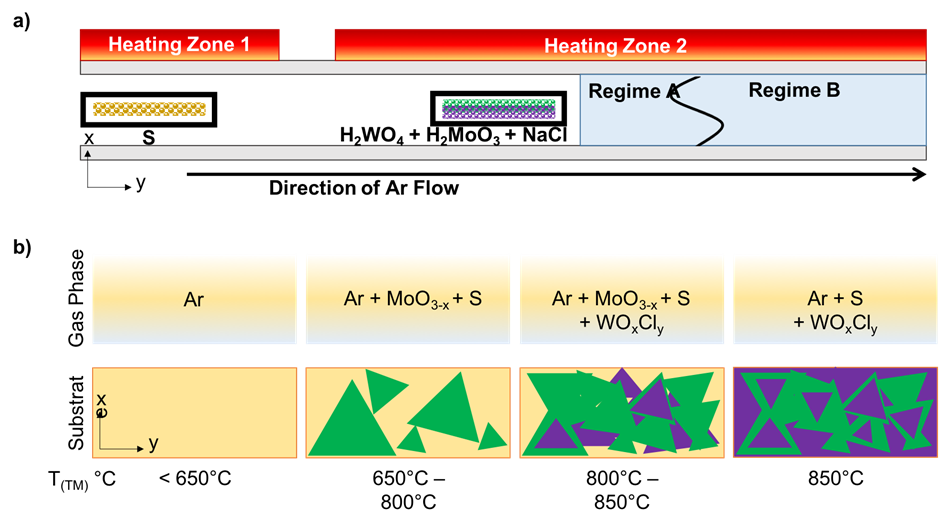
\includegraphics[scale=0.5]{Heterostructures/CVDGrowthSetup.png}
		\caption{Schematic of the CVD growth process for tunable heterostructure and alloy synthesis; a) representation of the precursor positions, heating zone, and substrate in space; and b) simplified representation of the gas phase components and nucleation and growth on $Si/SiO_2$ (green colour = Mo region;  purple colour = W region).}
		\label{fig:HeterostructureCVDGrowthSetup}
	\end{center}
\end{figure}

\begin{figure}[h]
	\begin{center}
		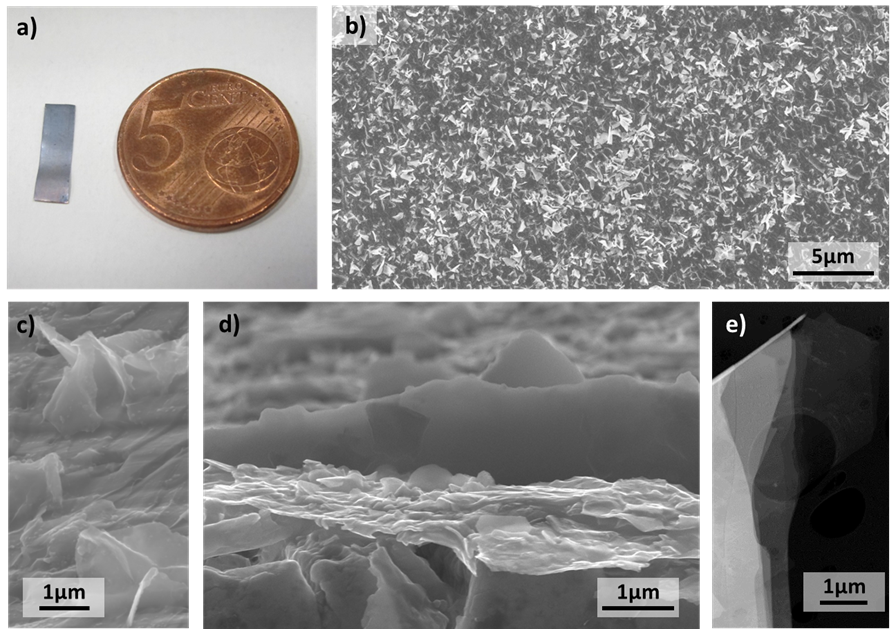
\includegraphics[scale=0.5]{Heterostructures/SEMImages.png}
		\caption{(a) Photograph of $MoS_2/WS_2$ heterostructure grown on gold; (b) scanning electron micrographs (SEM) of $MoS_2/WS_2$ heterostructures grown on gold showing continuous distribution of material; (c) side; (d) cross-sectional SEM image of combined lateral and vertical growth modes; and (e) STEM image of the edge of a flake.}
		\label{fig:HeterostructureSEMImages}
	\end{center}
\end{figure}

The dual growth conformation where a vertical geometry of the flakes supersedes the initially formed flakes parallel to the substrate, can be more easily achieved on Gold rather than $SiO_2$, due to the high capture rate of sulphur during the nucleation stage of CVD growth \cite{Gao2015}. This ensures good adhesion to the substrate by the conformal flakes (Figure \ref{fig:HeterostructureSEMImages} b) and a high available surface area by the flakes grown perpendicular to the substrate (Figure \ref{fig:HeterostructureSEMImages} c-e). Further, the exceptionally large lateral flakes size are retained despite this change in nucleation and growth mode (Figure \ref{fig:HeterostructureSEMImages} d, e).

%%%

A $WS_2$/$MoS_2$ heterostructure has been prepared by one step growth CVD. As a first step the heterostructure has been grown on $SiO_2/Si$ using parameters developed for monolayer growth. An optical micrograph of a select area of the sample can be seen in Figure \ref{fig:HeterostructureOMSi}. The sample contains large areas of monolayer and bilayer TMDCs with some very small flake of bulk material. Overall the material coverage is quite high.

The sample was then characterised using Raman and PL spectroscopy. A measurement of Raman spectrum was taken from heterostructure and as seen in Figure \ref{fig:HeterostructureRamanSpectrum} a distinct spectrum of $WS_2$ and $MoS_2$ can be distinguished. The Raman peak positions are 350.1 $cm^{-1}$, 382 $cm^{-1}$, 408.3 $cm^{-1}$ and 417.7 $cm^{-1}$ which can ascribed to $WS_2$ $E^1_{2g}$, $MoS_2$ $E^1_{2g}$, $MoS_2$ $A_{1g}$ and $WS_2$ $A_{1g}$ respectively. Those peak position correspond to multi layers of the individual materials which indicates a certain level of interaction between the layers.

\begin{figure}[h]
	\begin{center}
		\includegraphics[scale=0.5]{Heterostructures/OmSi.png}
		\caption{Optical micrograph of $WS_2/MoS_2$ heterostructure on $SiO_2/Si$}
		\label{fig:HeterostructureOMSi}
	\end{center}
\end{figure}


\begin{figure}[h]
	\begin{center}
		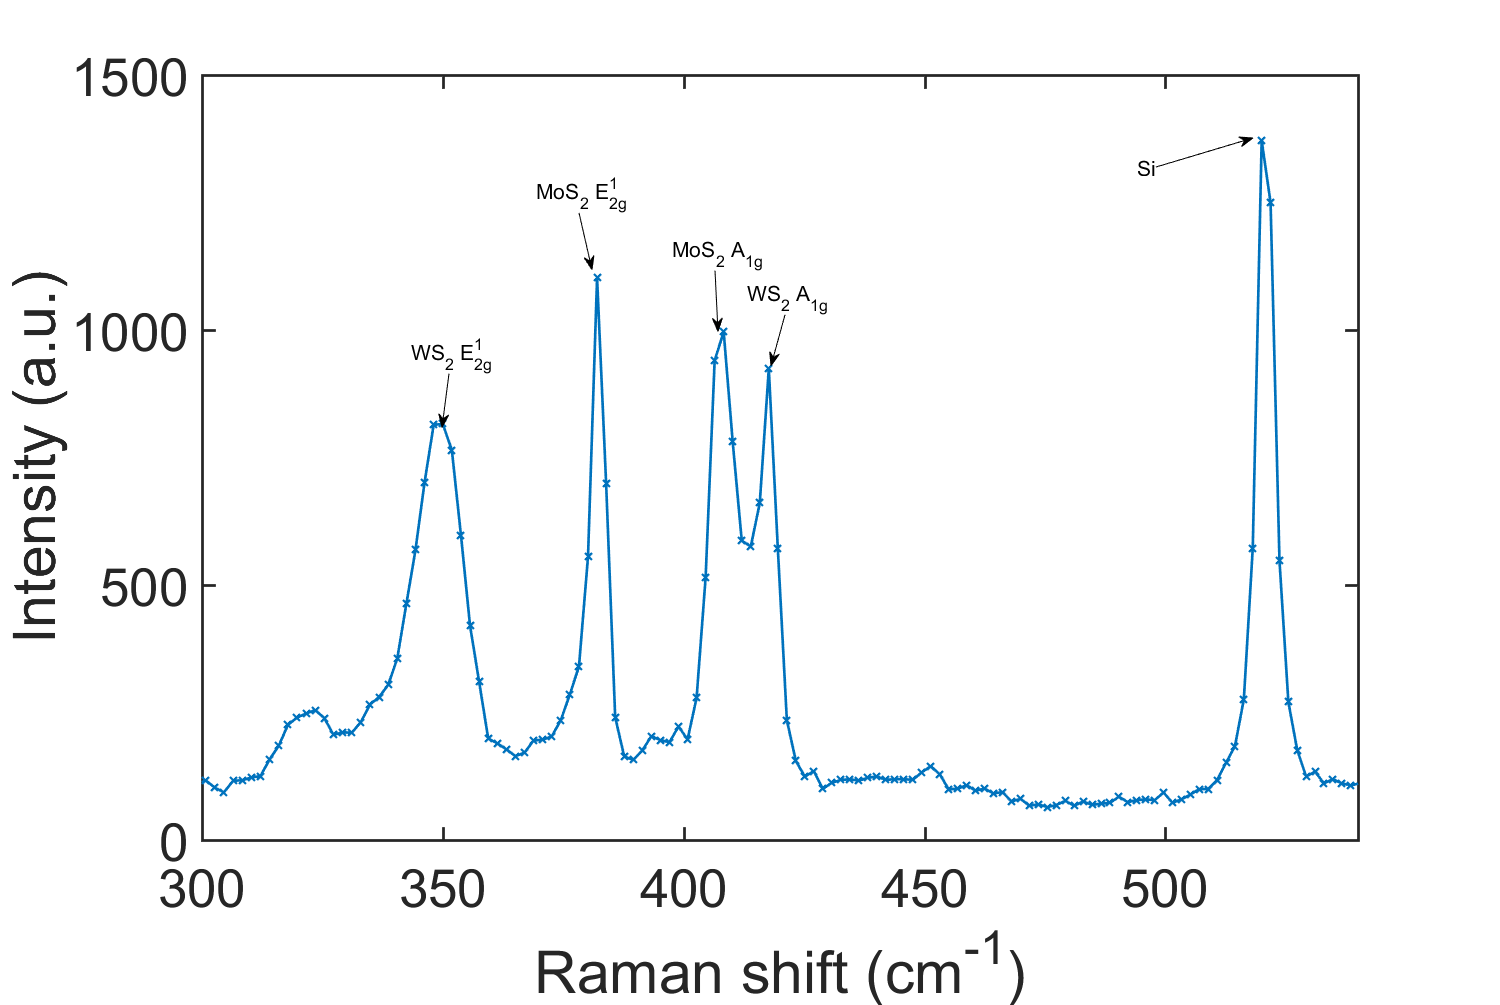
\includegraphics[scale=0.3]{Heterostructures/RamanSpectrum2.png}
		\caption{Raman spectrum of $WS_2$/$MoS_2$ heterostructure}
		\label{fig:HeterostructureRamanSpectrum}
	\end{center}
\end{figure}

There is a monolayer and bilayer $MoS_2$ found around the heterostructure area with no $WS_2$ grown  indicating that the $WS_2$ flake has grown on top of the $MoS_2$ layer. The area surrounding the heterostructure shows a spectrum as seen in Figure \ref{fig:HeterostructuresRamanSpectraMonoBi}. 
\newpage

\begin{figure}[h]
	\begin{center}
		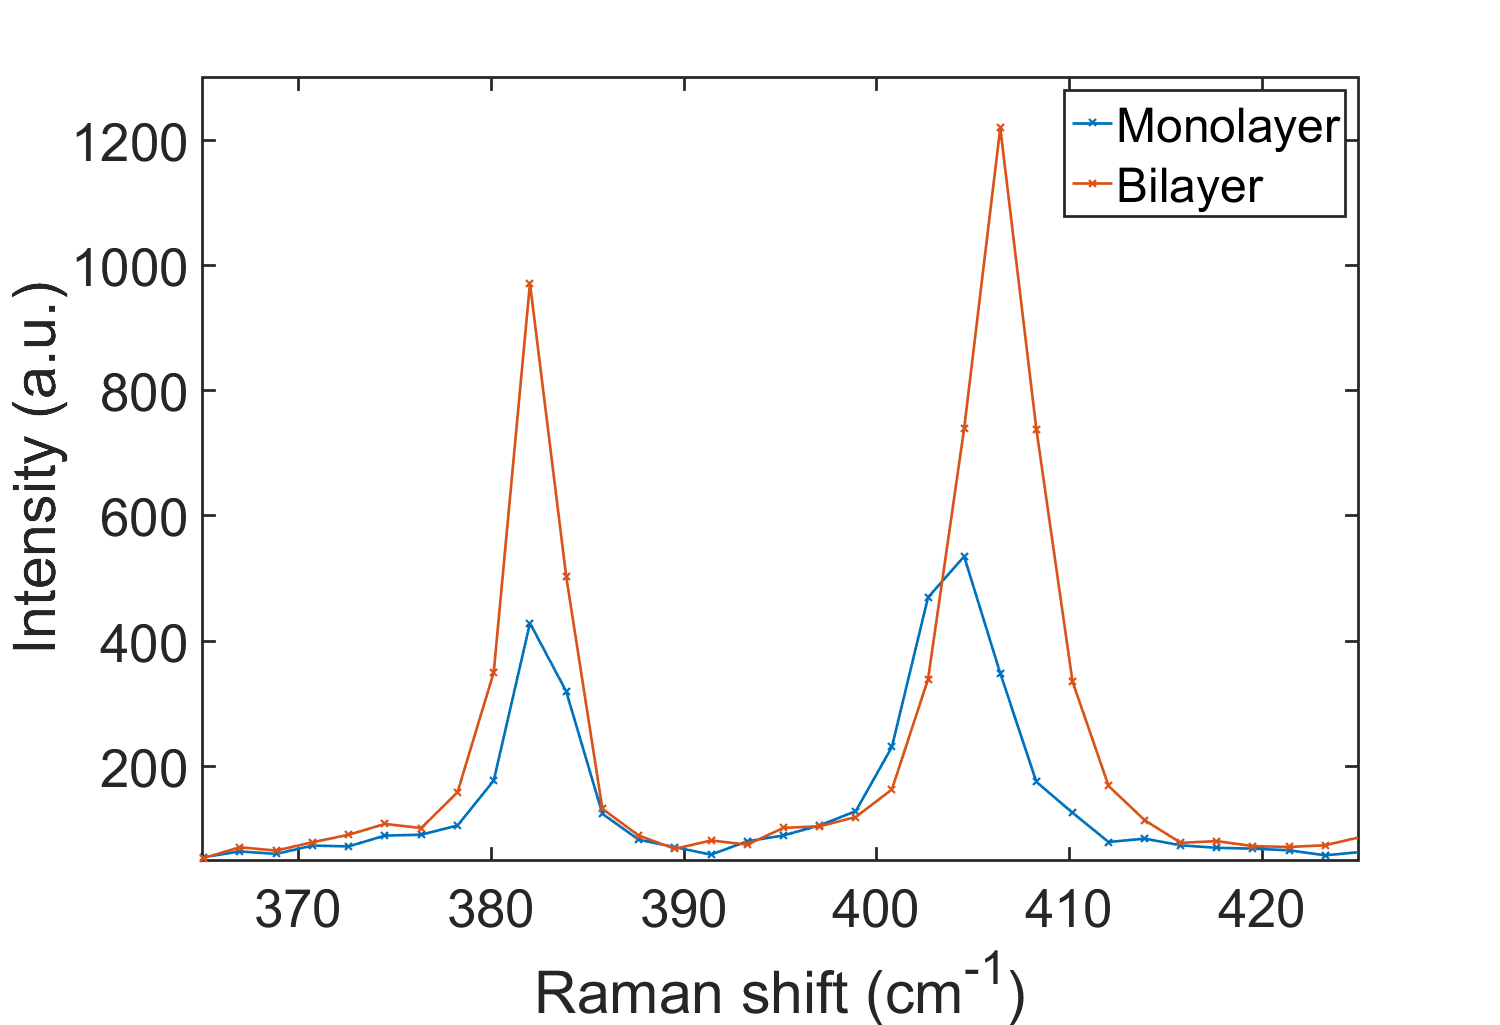
\includegraphics[scale=0.3]{Heterostructures/RamanSpectraMonoBi2.png}
		\caption{Raman spectra of mono an bilayer $MoS_2$}
		\label{fig:HeterostructuresRamanSpectraMonoBi}
	\end{center}
\end{figure}

The positions of the peaks are 382.7 $cm^{-1}$ and 404 $cm^{-1}$ for the monolayer and 382.4 $cm^{-1}$ and 406.4 $cm^{-1}$ for the bilayer.

The sample was then mapped using Raman spectroscopy. As seen in Figure \ref{fig:HeterostructuresRamanIntensityE} the intensity of $E^1_{2g}$ peak varies across the mapped area for both $WS_2$ and $MoS_2$. The more intense areas indicate more layers of $WS_2$ which is placed on top of $MoS_2$. Where the intensity of $WS_2$ $E^1_{2g}$ peak is higher and therefore there is more layers of $WS_2$ the intensity of $MoS_2$ $E^1_{2g}$ is reduced. 

\begin{figure}[h]
	\begin{center}
		\begin{subfigure}[b]{0.45\textwidth}
			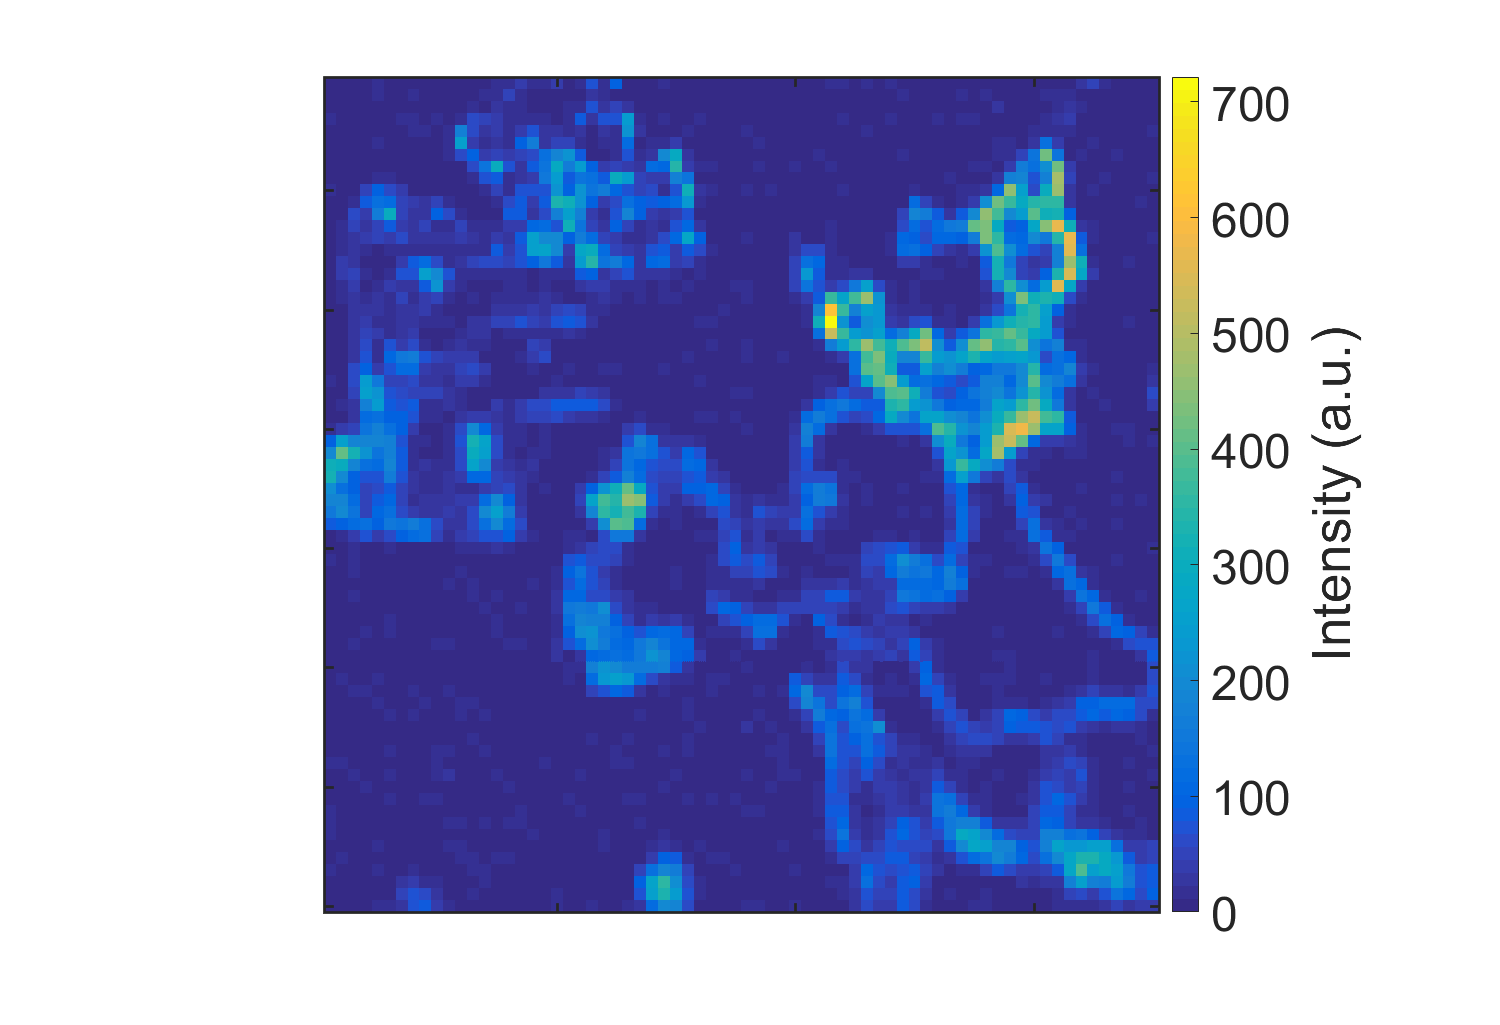
\includegraphics[width=\textwidth]{Heterostructures/RamanIntensityMapEWS2.png}
			\caption{$WS_2$}
			\label{fig:HeterostructuresRamanIntensityEWS2}
		\end{subfigure}
		\begin{subfigure}[b]{0.45\textwidth}
			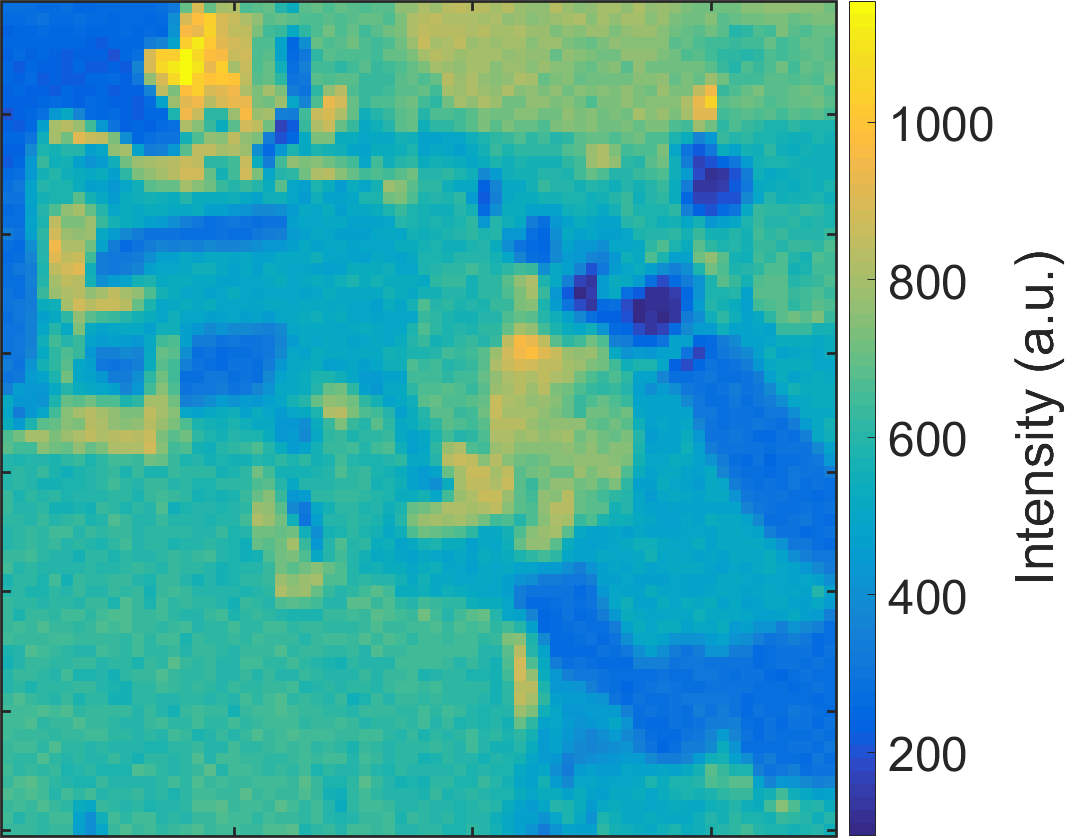
\includegraphics[width=\textwidth]{Heterostructures/RamanIntensityMapEMoS2.png}
			\caption{$MoS_2$}
			\label{fig:HeterostructuresRamanIntensityEMoS2}
		\end{subfigure}
		\caption{Map of Raman $E^1_{2g}$ peak intensity}
		\label{fig:HeterostructuresRamanIntensityE}
	\end{center}
\end{figure}

\begin{figure}[h]
	\begin{center}
		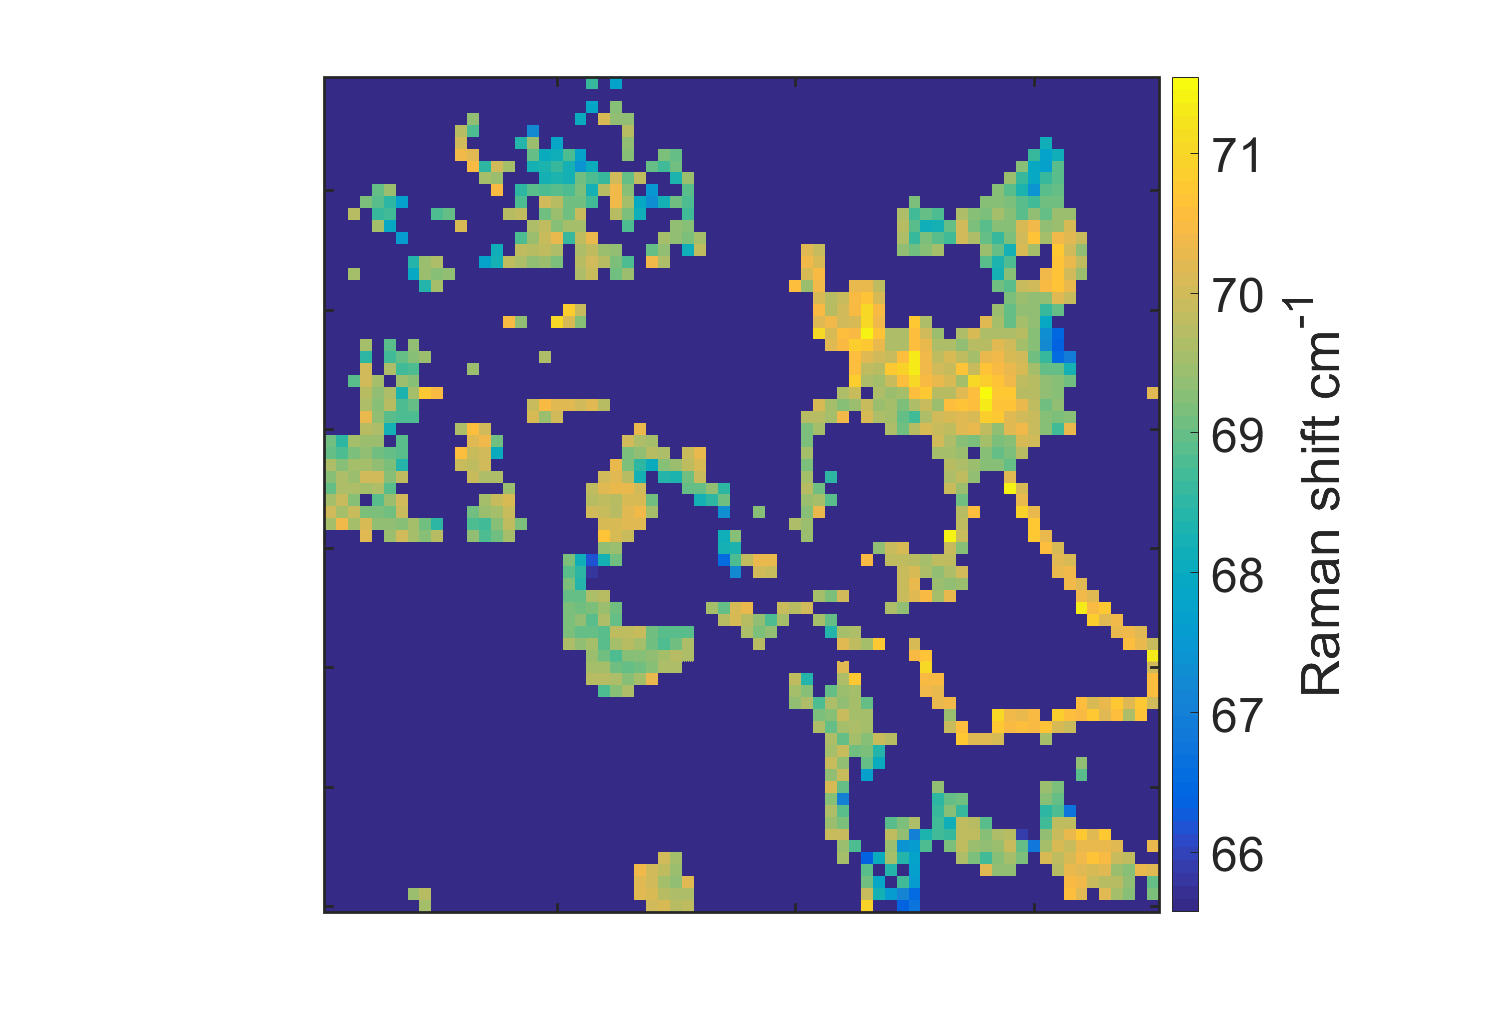
\includegraphics[scale=0.3]{Heterostructures/HeterostructureRamanDifferenceW.png}
		\caption{Difference between $WS_2$ $A_{1g}$ and $E^1_{2g}$ peak position}
		\label{fig:HeterostructuresRamanDifferenceW}
	\end{center}
\end{figure}

To better estimate the number of layers the difference between $A_{1g}$ and $E^1_{2g}$ peak positions has been also calculated. By excluding the bulk flakes and leaving the flakes with less or equal to 3 layers of $WS_2$ it can estimated that about 25\% of the area is covered with $WS_2/MoS_2$ heterostructure.

\begin{figure}[h]
	\begin{center}
		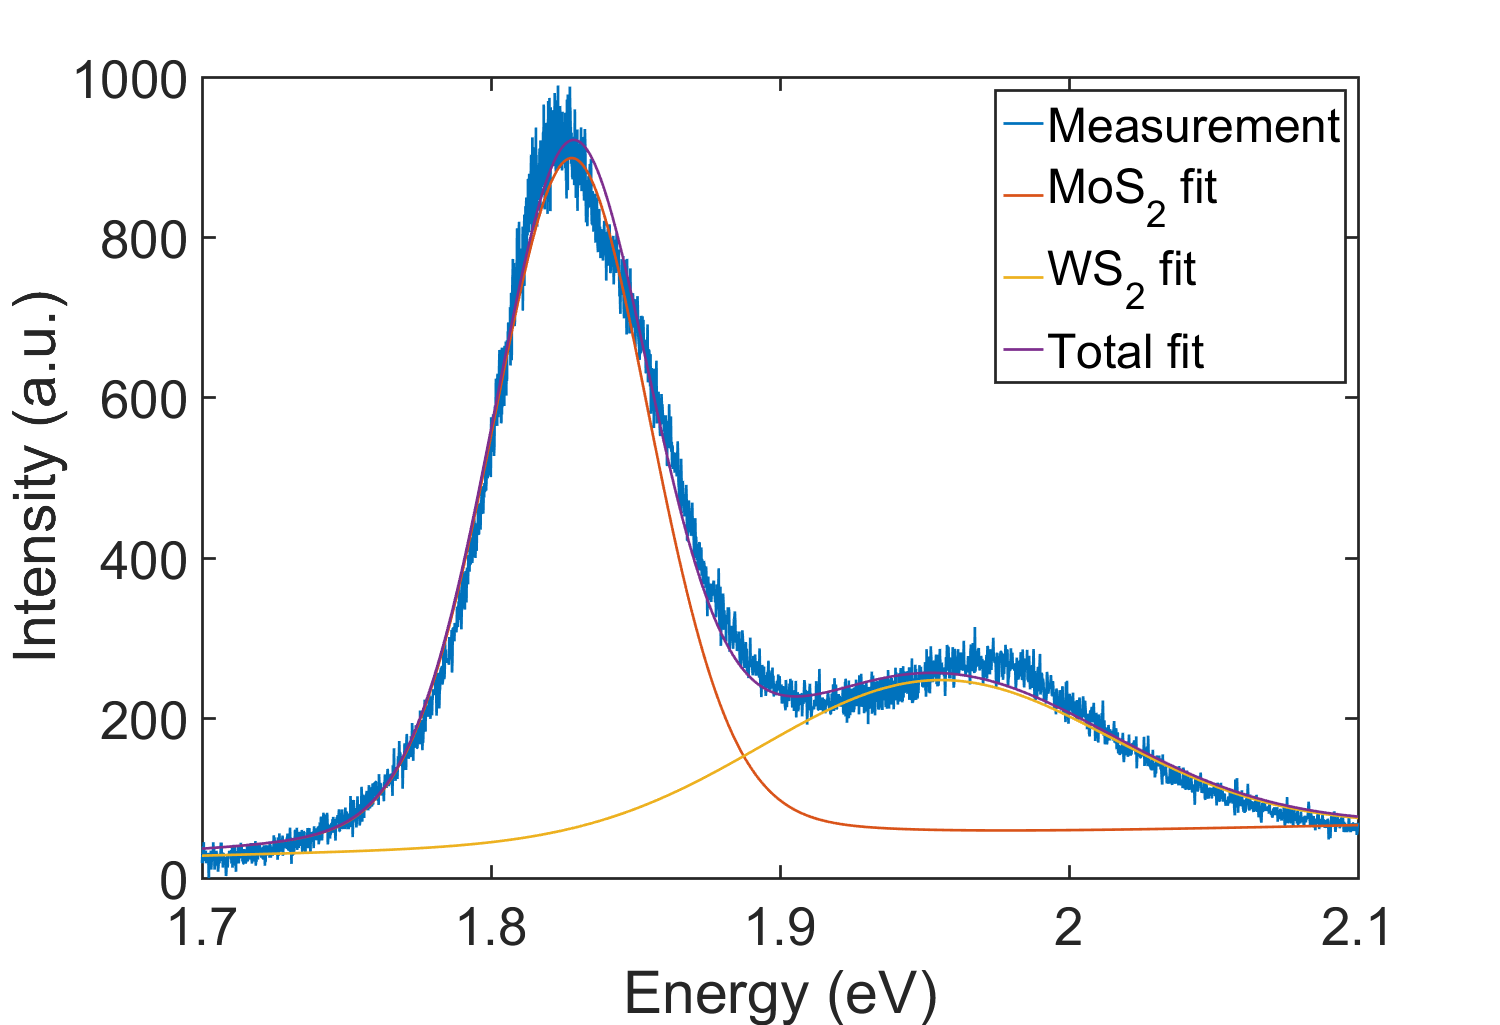
\includegraphics[scale=0.3]{Heterostructures/HeterostructurePLSpectrumFitted.png}
		\caption{PL spectrum of $MoS_2/WS_2$ heterostructure}
		\label{fig:HeterostructuresPLSpectrumFitted}
	\end{center}
\end{figure}

The PL spectrum of heterostructure can be seen in Figure \ref{fig:HeterostructuresPLSpectrumFitted}. There are two distinct peaks, one at at 1.824 eV and second at 1.971 eV. The position of the $MoS_2$ PL peak is consistent with the position of the monolayer $MoS_2$ as seen in Figure \ref{fig:HeterostructuresPLSpectrumMono} which is 1.825 eV. Those PL peaks from heterostructure therefore correspond to both $MoS_2$ and $WS_2$ monolayers indicating that the spectrum is additive. The $MoS_2$ peak is also much stronger than $WS_2$ despite the fact that isolated monolayer of $WS_2$ shows much stronger PL than a monolayer of $MoS_2$. The $MoS_2$ peak has a FWHM of 65.47 meV while the $WS_2$ PL peak has a FWHM of 142.4 meV. 

\begin{figure}[h]
	\begin{center}
		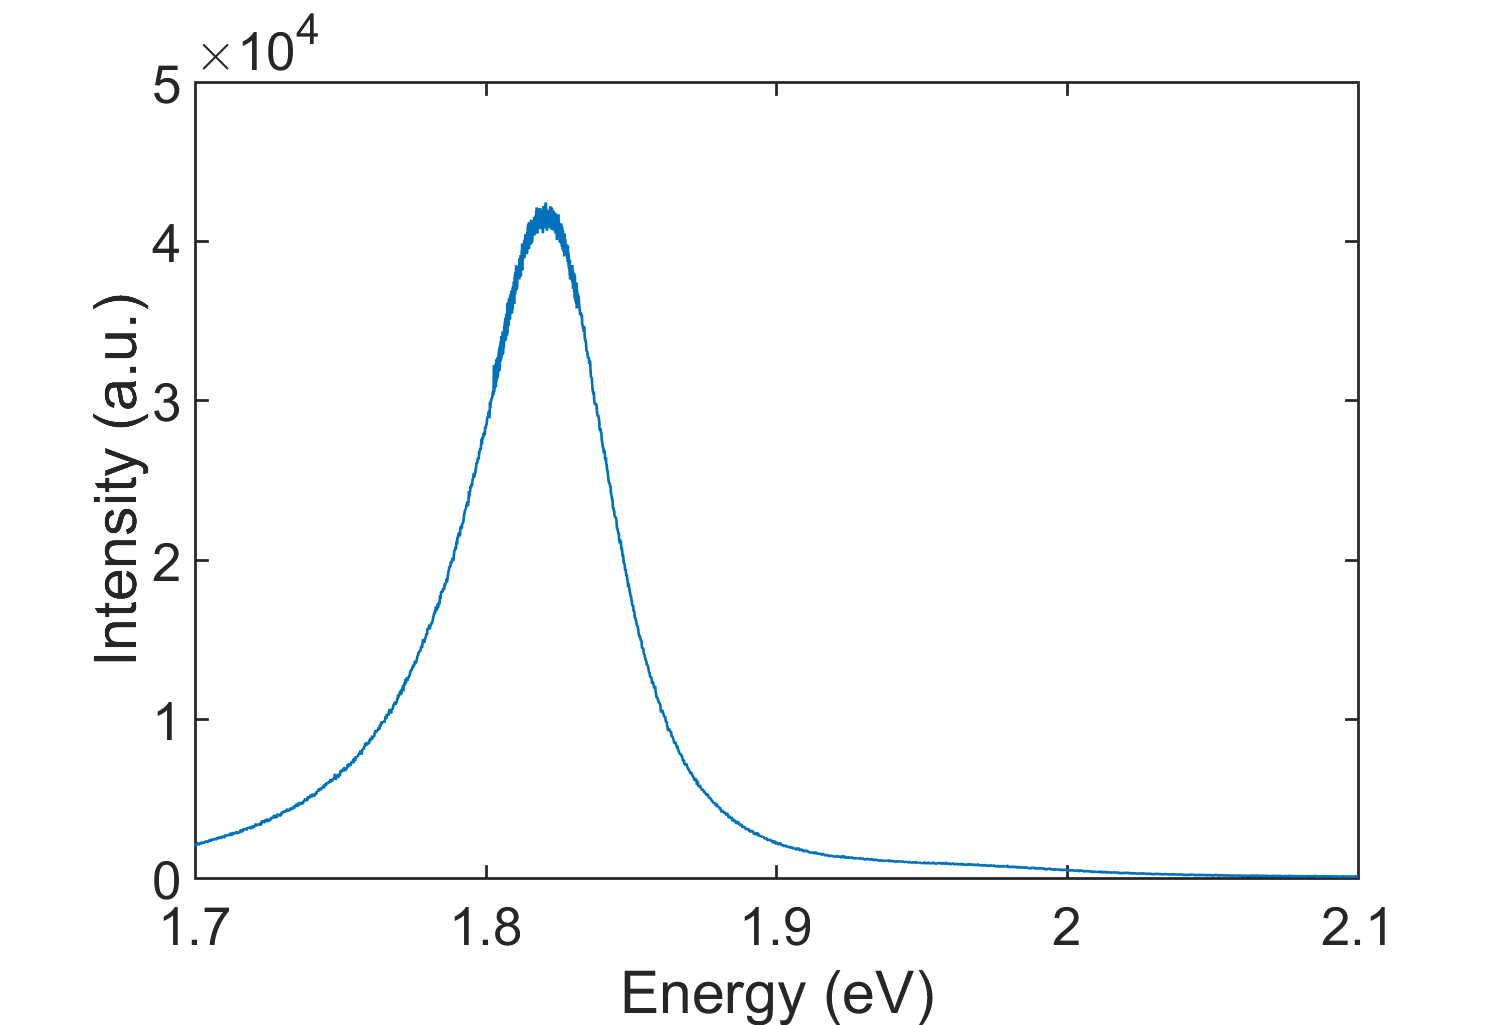
\includegraphics[scale=0.3]{Heterostructures/HeterostructurePLSpectrumMono.png}
		\caption{PL spectrum of $MoS_2$ monolayer}
		\label{fig:HeterostructuresPLSpectrumMono}
	\end{center}
\end{figure}

The sample was also mapped using PL spectroscopy as seen in Figure \ref{fig:HeterostructuresPLIntensityMap11}. The most intense PL can be observed in areas of monolayer $MoS_2$ and much weaker everywhere else. The position map of PL peaks from both $MoS_2$ and $WS_2$ can be seen further in Figure \ref{fig:HeterostructuresPLPositionsMaps}. Most of the PL of $MoS_2$ is around 1.82 eV with some 

\begin{figure}[h]
	\begin{center}
		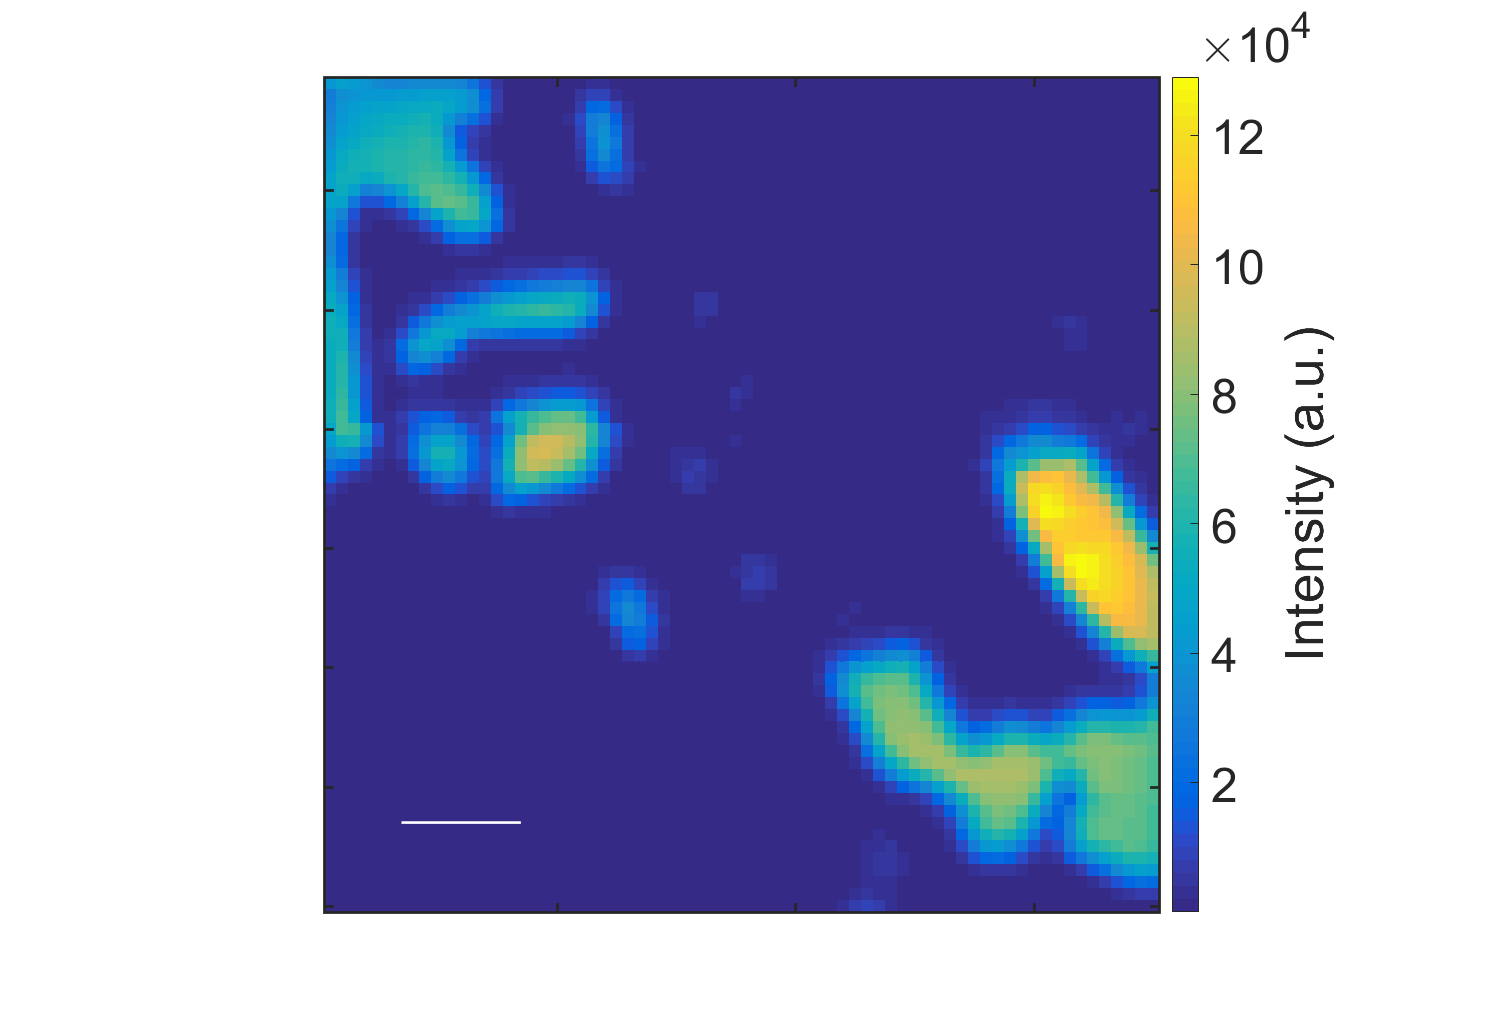
\includegraphics[scale=0.3]{Heterostructures/PLIntensityMap11.png}
		\caption{Integrated PL intensity}
		\label{fig:HeterostructuresPLIntensityMap11}
	\end{center}
\end{figure}

\begin{figure}[h]
	\begin{center}
		\begin{subfigure}[b]{0.5\textwidth}
			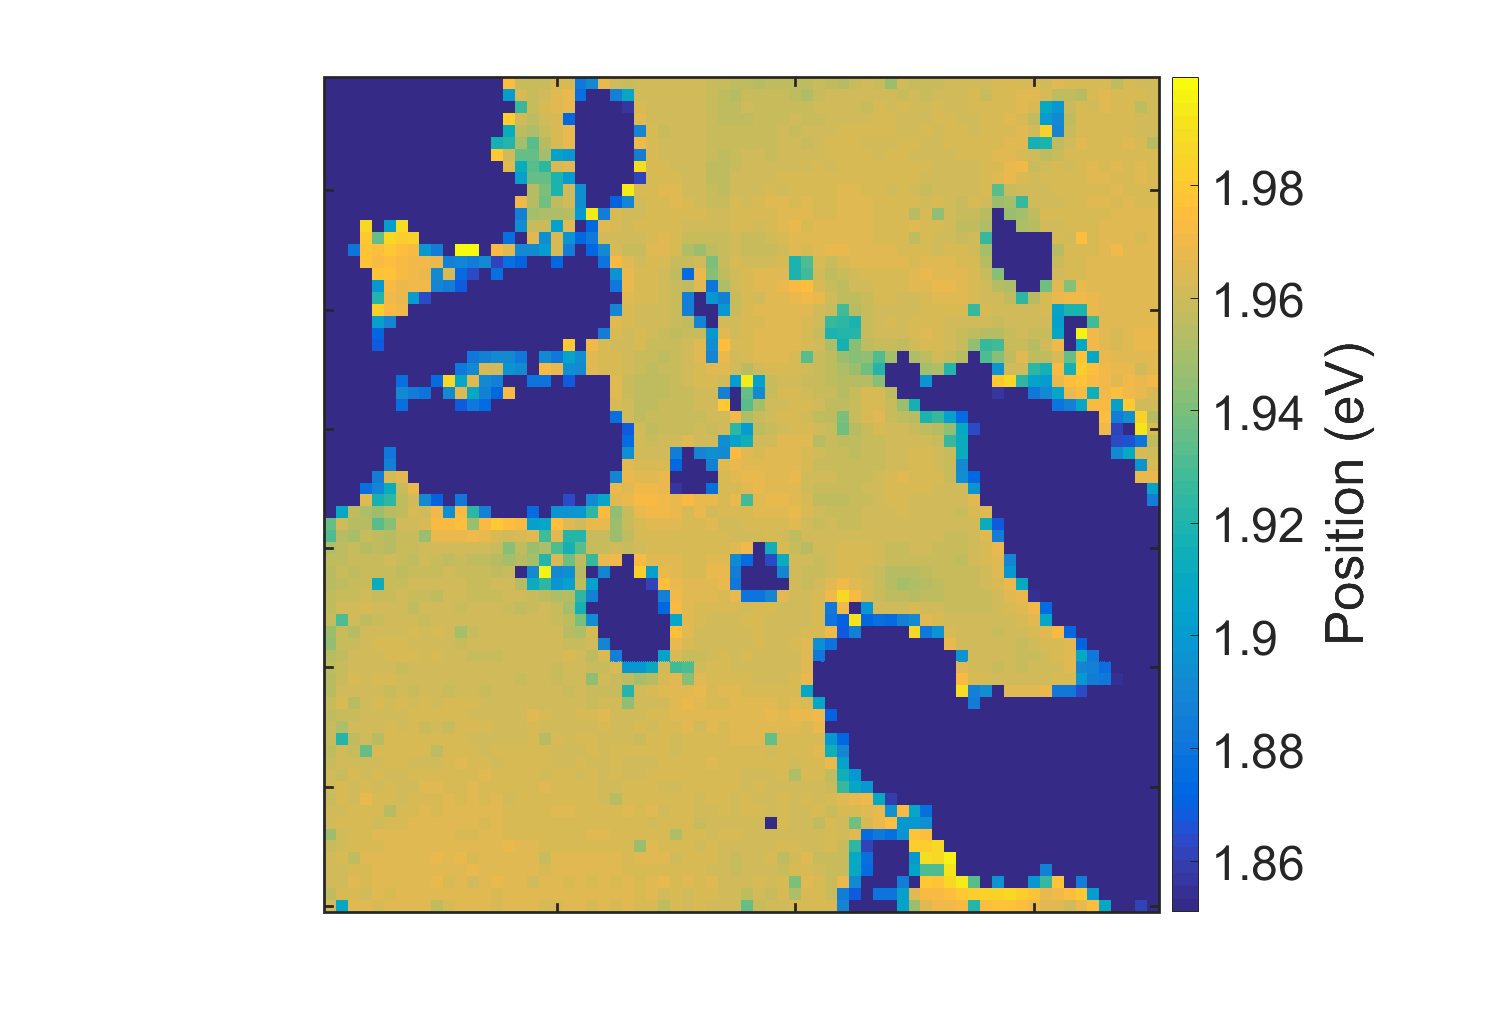
\includegraphics[scale=0.25]{Heterostructures/PLPositionMap21.png}
			\caption{PL position of the $MoS_2$ flake}
			\label{fig:HeterostructuresPLPosition21Map}
		\end{subfigure}
		\begin{subfigure}[b]{0.45\textwidth}
			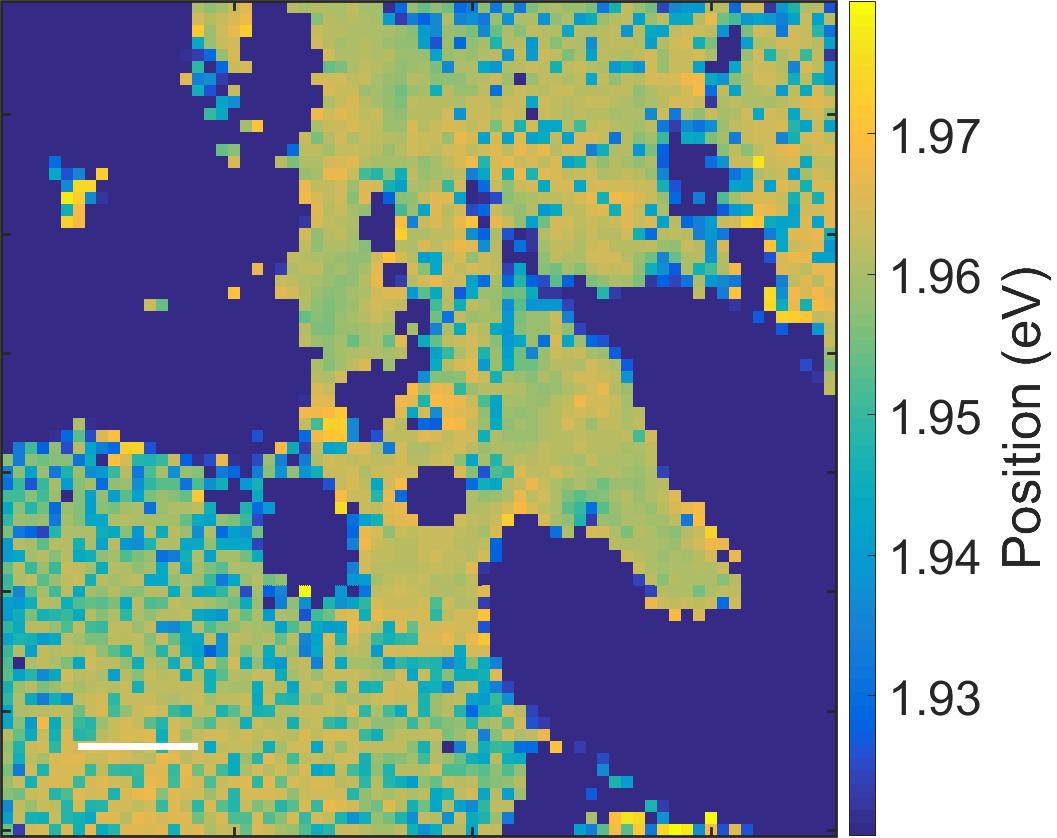
\includegraphics[scale=0.25]{Heterostructures/PLPositionMap22.png}
		\caption{PL position of the $WS_2$ flake}
		\label{fig:HeterostructuresPLPosition22Map}
		\end{subfigure}
		\caption{Map of PL peak positions}
		\label{fig:HeterostructuresPLPositionsMap}
	\end{center}
\end{figure}

The similar growth procedure was then used to grow $WS_2/MoS_2$ heterostructure on a gold substrate. As seen in Figure \ref{fig:HeterostructuresOMAu} the material coverage of the substrate is complete. The material also seems to be thick with irregular, rough surface. There are no visible triangles or continuous layers like seen in a $SiO_2/Si$ substrate. This is most likely due to vertical growth which can occur on gold substrate as opposed to $SiO_2/Si$ substrate.

\begin{figure}[h]
	\begin{center}
		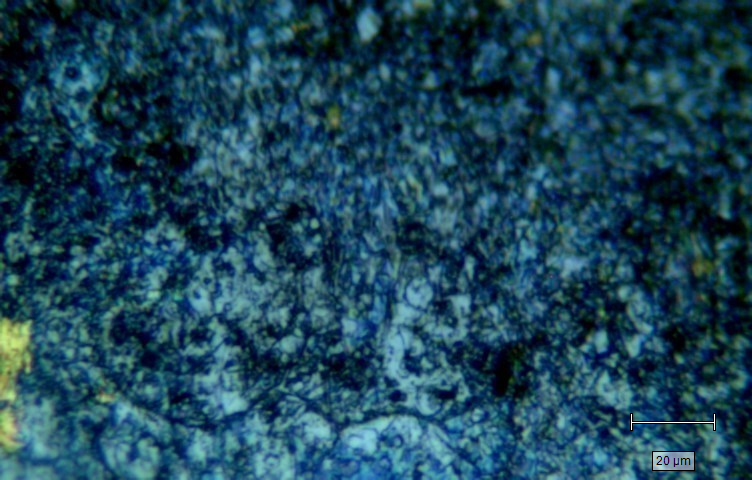
\includegraphics[scale=0.3]{Heterostructures/OMAu.png}
		\caption{Opitcal micrograph of the $WS_2/MoS_2$ grown on gold substrate}
		\label{fig:HeterostructuresOMAu}
	\end{center}
\end{figure}

The sample was then mapped using Raman spectroscopy. As seen in Figure \ref{fig:HeterostructureRamanSpectrumAu} the $WS_2$ and $MoS_2$ Raman peaks $E^1_{2g}$ and $A_{1g}$ can be identified.

\begin{figure}[h]
	\begin{center}
		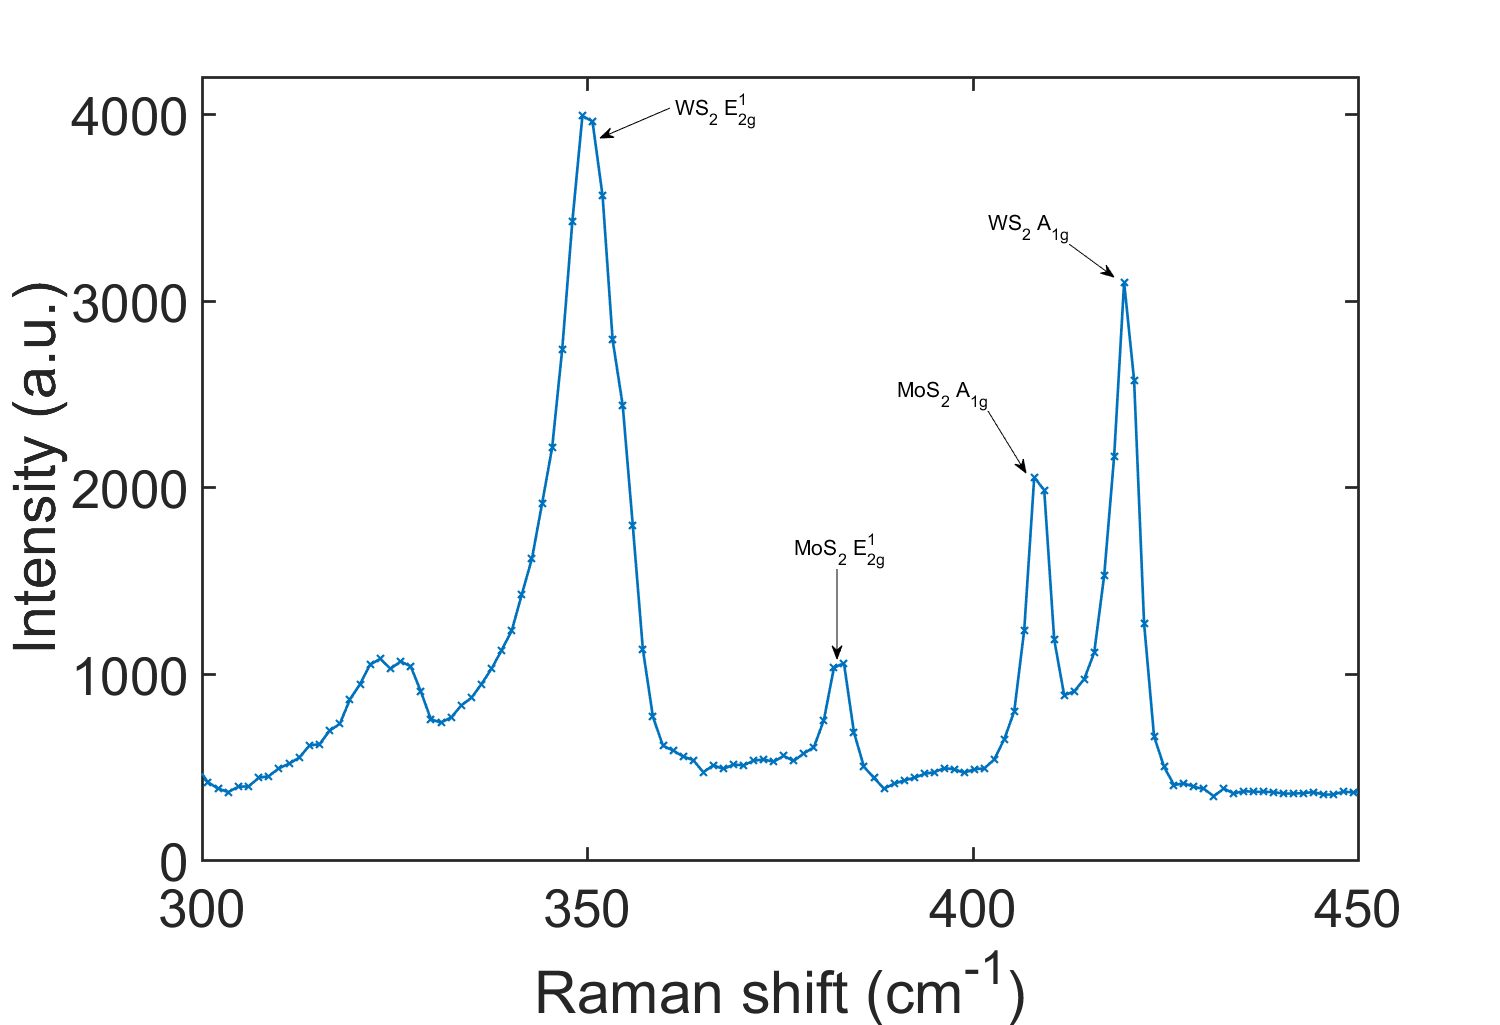
\includegraphics[scale=0.3]{Heterostructures/RamanSpectrumAu.png}
		\caption{Raman spectrum of $WS_2/MoS_2$ on gold substrate}
		\label{fig:HeterostructuresRamanSpectrumAu}
	\end{center}
\end{figure}

As seen in Figure \ref{fig:HeterostructuresRamanIntensityEMaps} the $MoS_2$ $E^1_{2g}$ can be seen across the entire scanned area. On the other the $WS_2$ $E^1_{2g}$ peak can be seen less spread around. Additionally the areas with high intensity $WS_2$ $E^1_{2g}$ coincide with low intensity $MoS_2$ $E^1_{2g}$. It implies therefore that similarly to the $SiO_2/Si$ substrate the $WS_2$ grows on top of the $MoS_2$ which results in a weaker Raman signal from $MoS_2$ from areas where thick $WS_2$ has grown on top of the underlying $MoS_2$. 

\begin{figure}[h]
	\begin{center}
		\begin{subfigure}[b]{0.5\textwidth}
			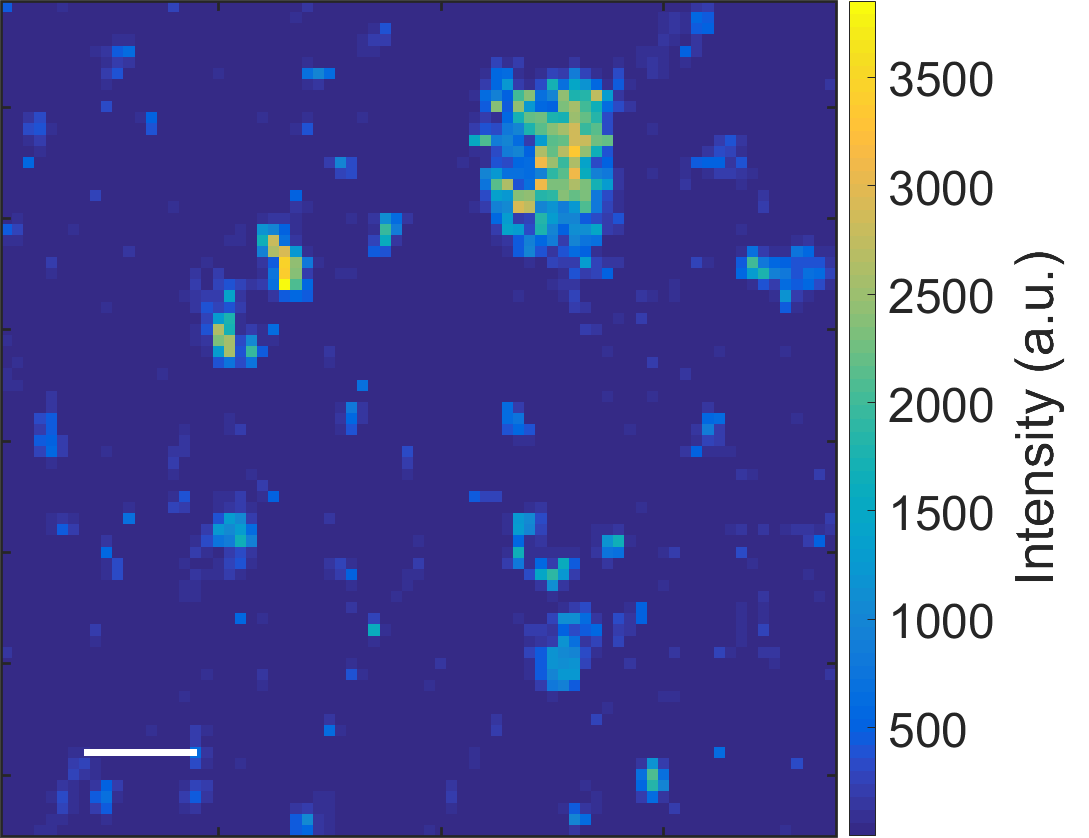
\includegraphics[scale=0.25]{Heterostructures/HeterostructuresRamanIntensityEWAu.png}
			\caption{$WS_2$ $E^1_{2g}$ peak intensity map}
			\label{fig:HeterostructuresRamanIntensityEWAu}
		\end{subfigure}
		\begin{subfigure}[b]{0.45\textwidth}
			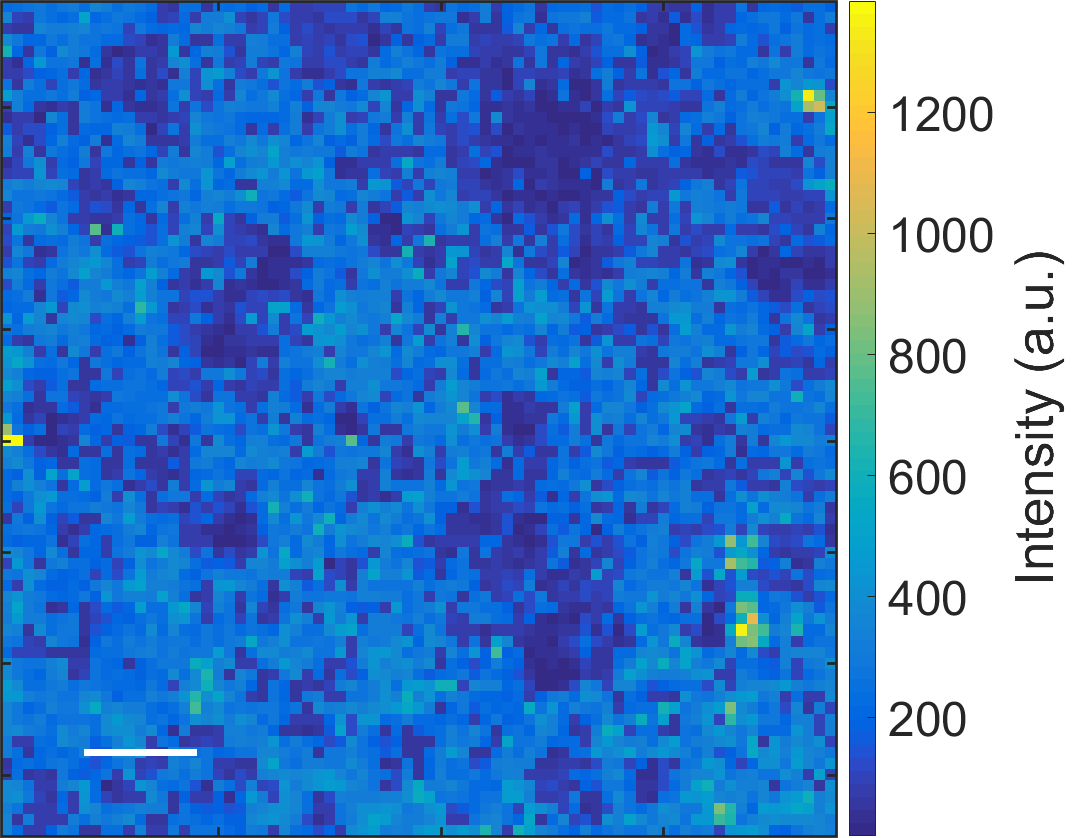
\includegraphics[scale=0.25]{Heterostructures/HeterostructuresRamanIntensityEMoAu.png}
			\caption{$MoS_2$ $E^1_{2g}$}
			\label{fig:HeterostructuresRamanIntensityEMoAu}
		\end{subfigure}
		\caption{Raman $E^1_{2g}$ intensity maps}
		\label{fig:HeterostructuresRamanIntensityEMaps}
	\end{center}
\end{figure}

The peaks positions for $WS_2$ are on average 349.1 $cm^{-1}$ and 418.5 $cm^{-1}$ for $E^1_{2g}$ and $A_{1g}$ respectively. Similarly for $MoS_2$ the peaks positions are 382.5 $cm^{-1}$ and 408.6 $cm^{-1}$ for $E^1_{2g}$ and $A_{1g}$ respectively. This indicates that both $MoS_2$ and $WS_2$ are mostly few layers thick. It can be estimated that in the measured area the $WS_2$ coverage and therefore the $WS_2$/$MoS_2$ heterostructure presence is at least 8{\%}.

Due to the gold substrate the PL is partially quenched which combined with weak PL signal coming from few layer $WS_2$ and $MoS_2$ makes it difficult to taken any meaningful measurement.

%%%

The fact that these flakes are epitaxial van der Waals heterostructures has been further proven by STEM energy dispersive X-ray spectroscopy (EDS) imaging (Figure \ref{fig:HeterostructuresSEMImagesFlake} d-g, Figure \ref{fig:HeterostructuresTEMImages}). Further, these analysis elucidate that the growth mechanism can be described as initial nucleation of $MoS_2$ flakes prior to $WS_2$ due to the lower transfer temperature (and higher volatility of gas borne intermediates) of the utilised molybdenum oxide hydrate [$MoO_3.H_2O$] precursor (750 {\degree}C) compared to the tungsten oxide hydrate [$WO_3.H_2O$] (850 {\degree}C) \cite{Sahoo2018}\cite{Freedman1959}. 

\begin{figure}[h]
	\begin{center}
		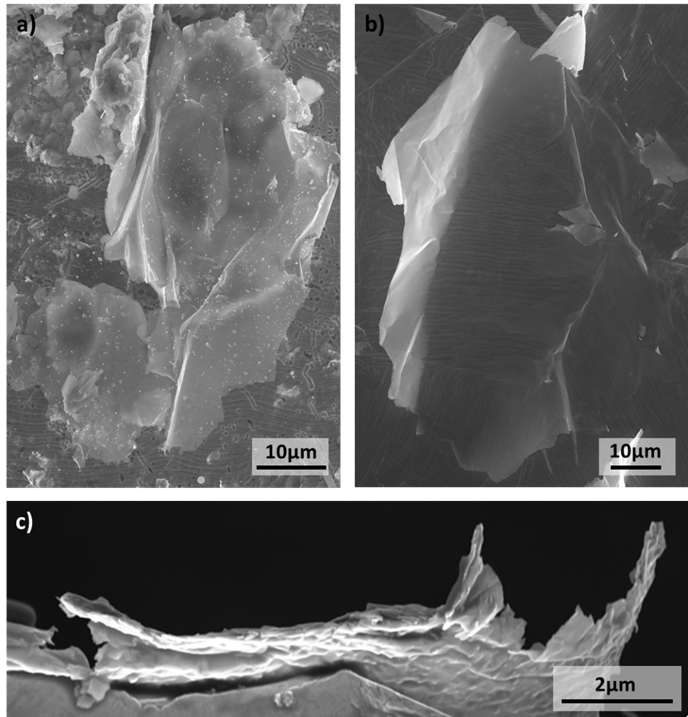
\includegraphics[scale=0.3]{Heterostructures/SEMImagesFlake.png}
		\caption{Scanning electron micrograph of (a,b) large lateral size flakes; and (c) cross-sectional area on gold foil}
		\label{fig:HeterostructuresSEMImagesFlake}
	\end{center}
\end{figure}

\begin{figure}[h]
	\begin{center}
		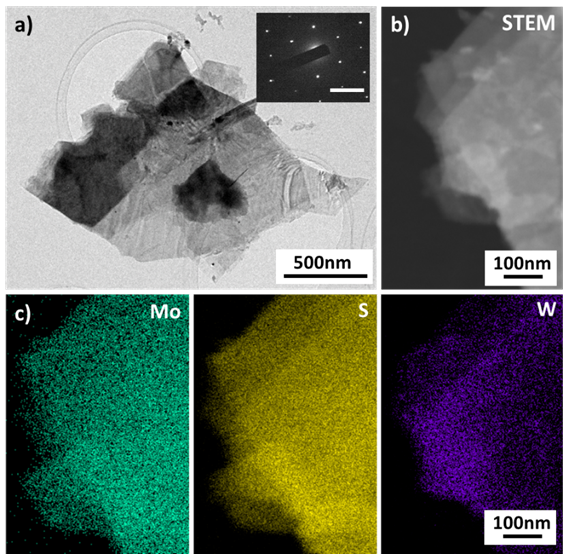
\includegraphics[scale=0.3]{Heterostructures/TEMImages.png}
		\caption{(a) Transmission electron micrograph of heterostructures flakes exfoliated via bath sonication in ethanol, post PEC characterization (inset: diffraction pattern taken from a molybdenum-rich area of the flake, scale bar = 5 $nm^{-1}$); (b) ADF-STEM image used for EDS spectral mapping; and (c) EDS spectral maps of intensity for Mo, S, W and the corresponding to (b) W and Mo localization in individual stacked flakes.}
		\label{fig:HeterostructuresTEMImages}
	\end{center}
\end{figure}

\begin{figure}[h]
	\begin{center}
		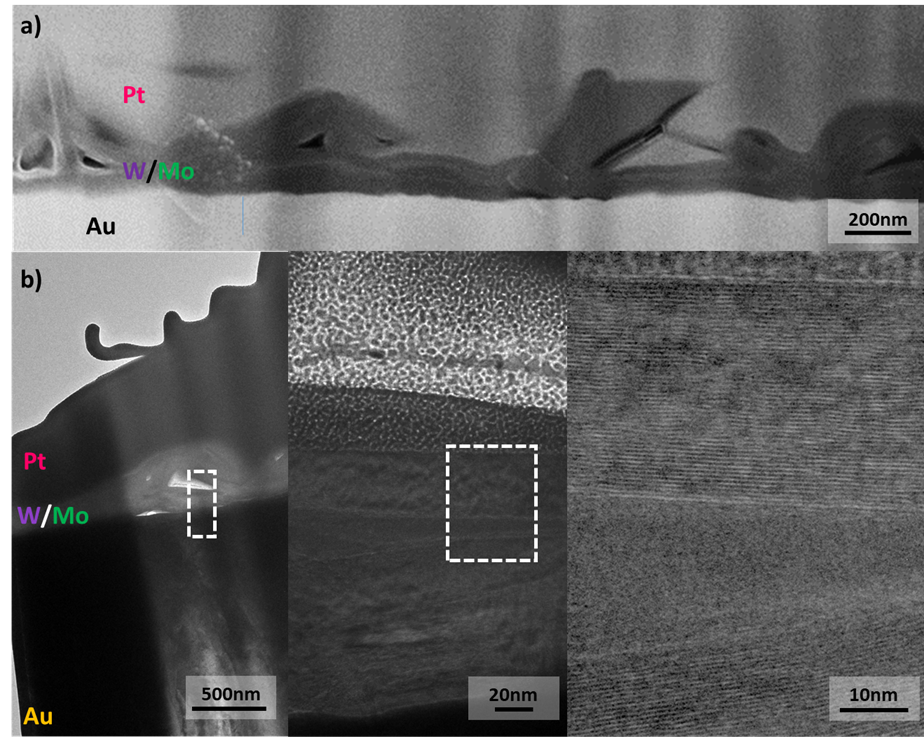
\includegraphics[scale=0.3]{Heterostructures/FIBTEMSEM.png}
		\caption{TEM images of FIB-extracted sample attained using the lift-out technique, showing film thickness of less than 1${\mu}m$, vertical growth modes, and crystalline flakes; (a) SEM image (visible squares correspond to HRTEM and STEM/EDS regions); and (b) sequential TEM images at increasing magnification.}
		\label{fig:HeterostructuresFIBTEMSEM}
	\end{center}
\end{figure}

\begin{figure}[h]
	\begin{center}
		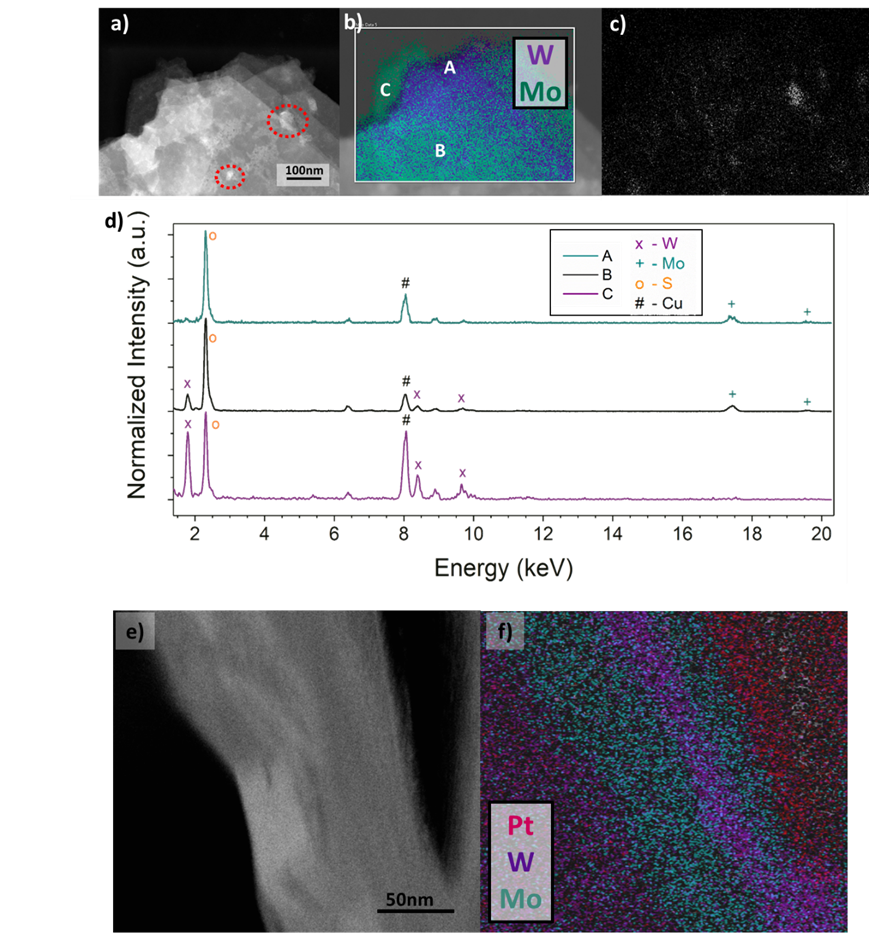
\includegraphics[scale=0.3]{Heterostructures/STEMEDS.png}
		\caption{(a) STEM image of 2D crystal heterostructure post-PEC cycling; (b) overlap of EDS maps of W (purple) and Mo (cyan) highlighting localization of both elements in separate yet overlapped layers; (c) oxygen EDS signal post-PEC; (d) individual EDS spectra extracted from regions A, B, and C as highlighted in (b); (e) FIB-STEM of an equivalent flake structure to (a); and (f) EDS map of (d) showing W localization within Mo layers (S not shown for clarity). It should be noted that assignment of W, Au, and S signal required deconvolution using Aztec EDS software due to the overlap between W, Au, and S lines.}
		\label{fig:HeterostructuresSTEMEDS}
	\end{center}
\end{figure}

\begin{figure}[h]
	\begin{center}
		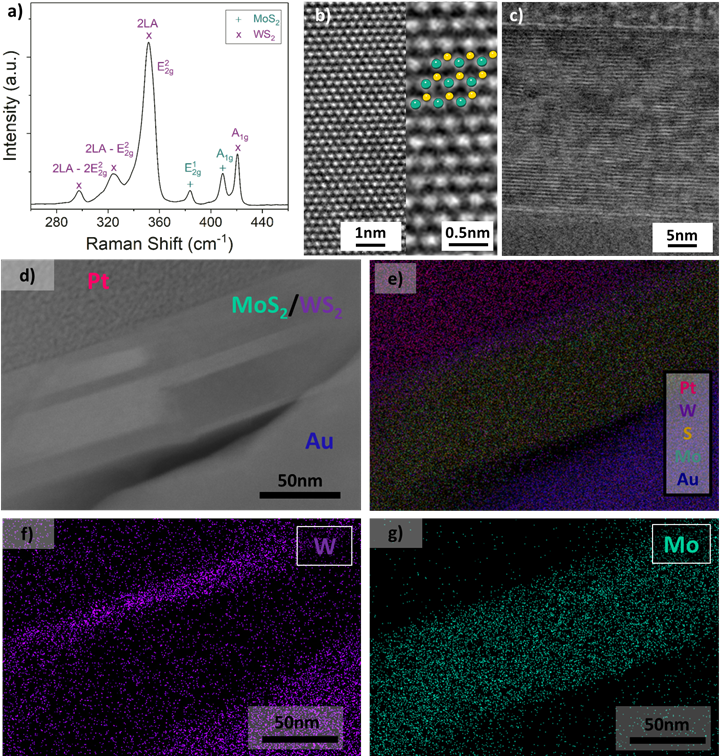
\includegraphics[scale=0.3]{Heterostructures/FIBSTEMEDS.png}
		\caption{(a) Raman spectrum with independent modes of $WS_2$ and $MoS_2$ representative of heterostructure formation; (b) high-resolution TEM image with an atomic model overlaid showing crystallinity; (c) cross-sectional TEM obtained from a FIB cut sample; FIB-STEM-EDS mapping of a $MoS_2$/$WS_2$ heterostructure; d) STEM image; e) composite overlaid map showing sequentially: substrate (Au), $MoS_2$ layer, $WS_2$ layer; and protective Pt coating; and individual EDS maps for f) W; and g) Mo.}
		\label{fig:HeterostructuresFIBSTEMEDS}
	\end{center}
\end{figure}

High-resolution TEM imaging demonstrates a high crystalline nature of the basal planes of the heterostructures formed by atomic columns with the inter-planar distances of 2.6 \r{A} consistent with that of the (100) planes of 2H $MoS_2$ and $WS_2$ (2.73 \r{A}, the difference of 0.13 \r{A} falls within the expected error range) (Figure \ref{fig:HeterostructuresFIBSTEMEDS} b). Cross-sectional imaging along [002] direction additionally confirms a high crystalline nature of the lateral planes of the heterostructures. From SEM imaging, we can ascertain that the average sample thickness of the lateral growth mode is 80 $\pm$ 30 nm while the vertical growth modes reaches up to 400 nm vertically (Figure \ref{fig:HeterostructuresFIBTEMSEM}). STEM-EDS performed on individual, multi-layered, heterostructure flakes after photo-electrochemical cycling showed chemically pristine materials with individual sheets of $MoS_2$ (no W signal) and $WS_2$ (no Mo signal) within a single flake (Figure \ref{fig:HeterostructuresSTEMEDS}). The localized regions confirm the formation of individual sheets of MoS2 and WS2 within a single, epitaxial, van der Waals heterostructure.45 The majority of flakes studied showed strong W and Mo signals due to overlapping regions of the heterostructures. The produced epitaxial $MoS_2/WS_2$ heterostructure forms a type-II heterojunctions with a stepped band alignment, allowing for hole transfer from the $MoS_2$ to $WS_2$ and electron transfer from $WS_2$ to $MoS_2$, enhancing charge separation (Figure S7).\cite{Zhuang2013}\cite{Hong2014}\cite{Ma2018}. 
The PEC activity of the heterojunctions for water oxidation are reported in the Appendix of this thesis. 

\newpage
\section{Appendix}

The PEC activity was studied in 3.5\% w/v NaCl in DI water. Linear sweep voltammetry (LSV) was performed directly on as-synthesized samples with chopped illumination at 1.5 sun in both sweep directions, with visible bubbles appearing upon the electrode surface when illuminated at potentials >1.18 V vs RHE (Figure \ref{fig:HeterostructuresCyclicVoltammetry} a, b, Figure S8). An early onset of measureable photocurrent at +0.48 V vs RHE was observed with the maximum on off ratio at +1.01 V vs RHE (Figure S8 a). A bare gold foil, which had been subjected to the CVD process without the addition of Mo, W, or S precursors, was used as a control and showed no catalytic activity for water oxidation. 

\begin{figure}[h]
	\begin{center}
		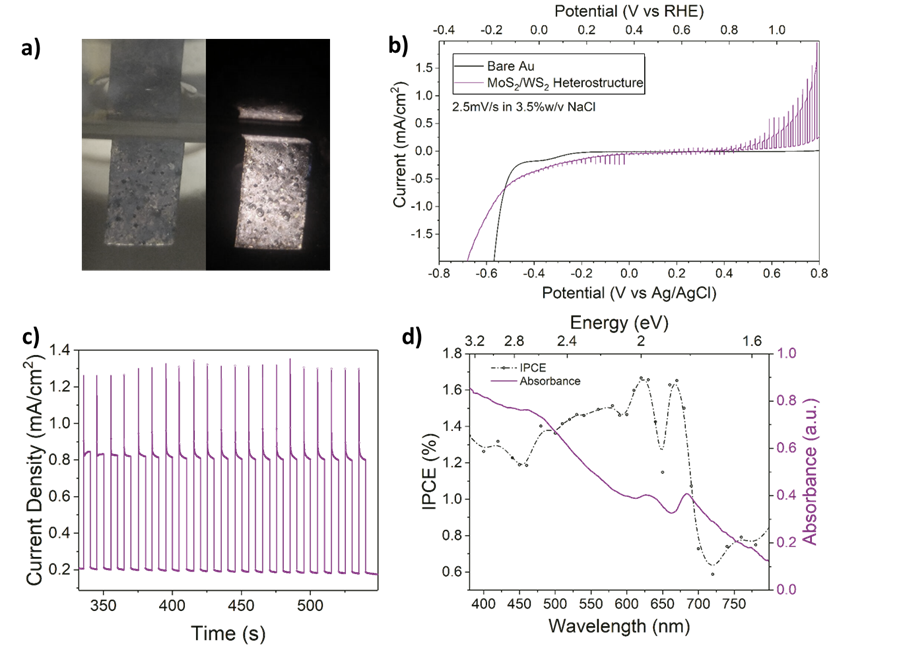
\includegraphics[scale=0.3]{Heterostructures/CyclicVoltammetry.png}
		\caption{Photoelectrochemical characterisation of MoS2/WS2 heterostructure on gold in 3.5\% w/v NaCl in DI water; (a) Photograph of active electrode at +0.75 V vs Ag/AgCl, left: no-illumination, right: illuminated, showing gas bubble formation; (b) linear sweep voltammetry at 2.5 mV/s from +0.8 to -0.8 V vs Ag/AgCl demonstrating the complete protection of the Au surface as minimal noble-metal hydrogen evolution is observed and negligible contribution of the substrate to either dark or photocurrent in the water oxidation region; (c) chronoamperometry at +0.75 V vs Ag/AgCl with chopped illumination at 0.2 Hz; and (d) photocurrent dependence on monochromatic light at +0.75 V vs Ag/AgCl and corresponding absorbance spectra of the heterostructures dispersed via sonication in ethanol.}
		\label{fig:HeterostructuresCyclicVoltammetry}
	\end{center}
\end{figure}

At potentials below +0.4 V vs RHE an inversion of the photocurrent was observed with significant instantaneous charge generation, however, negligible stable photocurrent was generated (Figure \ref{fig:HeterostructuresCyclicVoltammetry} b). This contribution arises due to the ambipolar characteristics of the TMDCs. In order to probe this effect, two stage chronoamperometry (CA) at -0.6 V vs Ag/AgCl and +0.75 V vs Ag/AgCl with chopped illumination was performed (Figure S8 b). The result of the chopped illumination at negative potentials was a slow increase in negative current flow upon illumination, which was recovered at approximately the same rate when the light source was blocked. When switched to positive potentials the previously described rapid water oxidation photocurrent was observed. 
CA performed at +1.129 V vs RHE, chosen to avoid oxygen bubble formation on the electrode surface, presented rapid charge generation immediately upon illumination followed by a stable photocurrent of 0.62 mA/cm2 at 1.5 sun illumination intensity (Figure \ref{fig:HeterostructuresCyclicVoltammetry} c) (0.4 mA/$cm^2$ at 1 sun, Figure S8 e). Sharp slopes in the chronoamperometry profiles collected  under chopped illumination were observed, suggesting a faster charge carrier recombination as compared to liquid phase processed material \cite{Pesci2017}. The observed fast kinetics of charge carrier recombination allowed for photocurrent to be obtained at frequencies up to 1 Hz, while a stable photocurrent under constant illumination was observed for over 10 minutes (Figure S8 e).  The photocurrent was confirmed to arise from the generation of oxygen through the use of an oxygen selective electrode, with an increase in the dissolved O2 concentration from 5 to 17 $\mu$mol/L upon illumination for 300 s (Figure S9). The Faradaic Efficiency (FE) for O2 generation was calculated to be 83 ± 15\%, indicating a high proportion of photogenerated holes being available to produce oxygen. The use of monochromatic light to obtain incident-photon-to-current efficiency (IPCE) demonstrates that the photocurrent mimics the reflectance spectra of the heterostructure, with IPCE of ~1.7\% at 690 nm, confirming that these heterostructures are capable of operation in the visible range (Figure \ref{fig:HeterostructuresCyclicVoltammetry}} d). The prominent features of both, reflectance and IPCE, are slightly red shifted from expected exciton positions for monolayer $MoS_2$ and $WS_2$ heterostructures (Table S1) \cite{Rigosi2015}.
The produced heterostructures demonstrates significant increase in efficiency compared to previously reported work on solution processed co-catalyst free TMDs for both hydrogen evolution (~0.1 \% IPCE) and water oxidation (~0.1 \% IPCE)\cite{Yu2015}\cite{Fu2015}. The attained photocurrent of 1.7 mA/$cm^2$ (increasing to 3.1 mA/$cm^2$ in $NaClO_4$, Figure S7 c) at 1.19 V vs RHE  in comparison to 5.35 mA/$cm^2$ for the best-in-class FeOOH-NiOOH/(W,Mo)-$BiVO_4$/$WO_3$ materials is promising, especially at lower IPCE values \cite{Shi2014a}. Indeed, the highest measured photocurrent of 1.7 mA/$cm^2$ at 0.79 V vs Ag/AgCl is directly comparable to high performance Mo or W/$BiVO_4$ composite systems 1.74 mA/$cm^2$ and 1.1 mA/$cm^2$ at 0.7 V and 1.1 V vs Ag/AgCl respectively.\cite{Hong2011}\cite{Pilli2011}. The FE of 83 ± 15\% for the CVD grown heterostructure is comparable to reported efficiencies for high performance electro- and photo- catalysts \cite{McCrory2015}.
This enhanced performance compared to analogous thin film hetrojunctions, \cite{Fu2015} as recently elucidated for exfoliated WSe2,\cite{Yu2017}\cite{Yu2017a} arises due to the highly crystalline nature of the flakes and their lateral size which is more than 100 times larger than the commonly used liquid phase exfoliated flakes. Large flakes sizes minimize recombination sites within our heterostructure and lead to the large grains overlapping with grain boundaries offset from one another. This offset allows for photo-generated charges to move laterally as well as vertically through the heterojunction with minimal recombination sites. These factors are proposed to minimize loss during charge transfer between $MoS_2$ and $WS_2$ layers. Finally, the relatively high volatility of utilized $H_2WO_4$ (and oxyhalide intermediates) ensures enriched $WS_2$ at the surface of the heterostructure (Figure \ref{fig:HeterostructuresSEMImagesFlake}) in contact with the electrolyte providing the ability for photo-generated holes, transferred in the $WS_2$, to directly interact with water molecules. Additionally, the observed kinetics of charge carrier recombination has similar time-scales to those reported by Yu et. al. using $WSe_2$ (and $WSe_2$/Pt heterostructures) as photo-cathodes for the hydrogen evolution reaction.\cite{Yu2015}\cite{Yu2017}\cite{Yu2016}.

